% Canonical, self-contained manuscript. Build with make -C whitepaper.
% The bibliography and vector diagram are inline for portable/native editing.
\documentclass[10pt,letterpaper,twocolumn]{article}
\usepackage[T1]{fontenc}
\usepackage{lmodern}
\usepackage[margin=0.75in]{geometry}
\usepackage{microtype}
\usepackage{amsmath,amssymb}
\usepackage{booktabs,array,tabularx}
\usepackage{xcolor}
\usepackage{tikz}
\usetikzlibrary{arrows.meta,positioning}
\usepackage{fancyhdr}
\usepackage{titlesec}
\usepackage{balance}
\usepackage{needspace}
\usepackage{url}
\usepackage[colorlinks=true,linkcolor=blue!40!black,citecolor=blue!40!black,urlcolor=blue!40!black]{hyperref}
\definecolor{ink}{HTML}{214E70}
\definecolor{pale}{HTML}{F1F5F8}
\hypersetup{pdftitle={RackNES: A Voltage-Controlled NES Emulator as a Musical Instrument},pdfauthor={Christian Kauten},pdfsubject={Retrospective instrument design and implementation report},pdfkeywords={NES, emulation, chiptune, modular synthesis, VCV Rack, musical interfaces}}
\setlength{\columnsep}{0.25in}
\setlength{\headheight}{14pt}
\setlength{\emergencystretch}{1.5em}
\titleformat{\section}{\large\bfseries\raggedright}{\thesection}{0.6em}{}
\titleformat{\subsection}{\normalsize\bfseries\raggedright}{\thesubsection}{0.6em}{}
\titlespacing*{\section}{0pt}{2.2ex plus 0.5ex minus 0.2ex}{1ex}
\titlespacing*{\subsection}{0pt}{1.7ex plus 0.4ex minus 0.2ex}{0.7ex}
\raggedbottom
\pagestyle{fancy}
\fancyhf{}
\fancyhead[L]{\small\textsc{RackNES}}
\fancyhead[R]{\small Technical report / September 2026}
\fancyfoot[C]{\thepage}
\newcommand{\code}[1]{\texttt{#1}}
\newcommand{\clip}{\operatorname{clip}}
\newcommand{\ceil}[1]{\left\lceil #1\right\rceil}
\title{\textbf{RackNES: A Voltage-Controlled NES Emulator\\as a Musical Instrument}}
\author{Christian Kauten\\Arhythmetic Units\\\small\href{mailto:arhythmetic.units@gmail.com}{arhythmetic.units@gmail.com}}
\date{September 30, 2026\quad /\quad Technical report, manuscript version 1}

\begin{document}
\twocolumn[\maketitle
\begin{abstract}
\noindent
RackNES embeds a Nintendo Entertainment System emulator in VCV Rack and
exposes console execution to a modular synthesizer patch. Controller gates,
clock-rate modulation, state recall, and individual audio outputs make the
running program part of the instrument. The CV Genie expander adds named,
game-specific memory writes, allowing patch signals to reach variables used
by game logic and music drivers. This retrospective describes the instrument's
foundations and implementation, organized around three intervention layers:
gameplay, execution, and memory. It explains the host-to-emulator timing
boundary, inherited sound synthesis, connection-dependent mixing, and the
difference between recalling machine state and replaying a recorded waveform.
The timing and snapshot boundaries reveal how implementation choices shape
the meaning of these controls. The contribution is a documented design for treating
an executable console program as patchable musical material, together with
engineering lessons about temporal coupling and state ownership. The account
is based on the released implementation and its documentation; it reports no
performance measurements or user study.
\end{abstract}
\par\vspace{0.7em}
\noindent\textbf{Keywords:} musical interfaces; console emulation; chiptune;
voltage control; state recall; modular synthesis.\par\vspace{1.5em}
]

\section{Introduction}
An NES game already contains a system for organizing sound: a program selects
events, advances musical sequences, assigns voices, and writes sound-chip
registers in response to changing game state. Bringing that program into a
modular synthesizer exposes a different kind of musical material from a bank
of isolated waveforms. A patch can act on the computation that produces sound,
as well as on the sound after it leaves the console.

RackNES implements this idea as a VCV Rack module. It loads a cartridge image,
runs an emulated CPU, picture processing unit (PPU), and audio processing unit
(APU), and presents the resulting video and five audio voices. Patch signals
can operate two controllers, change execution rate, request save and restore
operations, and suspend execution. CV Genie, an expander contributed by
\code{@anlexmatos}, supplies a further interface to selected memory locations.
The instrument's vocabulary therefore includes actions such as changing the
rate at which a game runs, returning to a saved execution state, and changing
a music driver's current song or sequence position.

The project changelog records an initial release in June 2020 and the Rack~2
port in February 2022. This report documents version~2.1.0 at source revision
\code{e8c99bf86295}, examined in September 2026~\cite{racknes}. The historical
implementation is the object of the account. Mathematical expressions below
describe its source-level behavior; patch examples describe possible uses of
its controls. Neither is presented as a runtime experiment.

The paper contributes an architectural account of whole-console integration,
a description of three distinct intervention layers, and an analysis of the
engineering boundaries that give those interventions their meaning. It makes
no priority claim for console instruments, game-based musical interfaces, or
clock manipulation. Its focus is the particular combination of a running game,
modular control, and access to the console's own voices.

\section{Foundations and Related Work}
\subsection{Voltage control and musical mappings}
Moog's account of voltage-controlled oscillators, amplifiers, and filters
established a modular vocabulary in which one signal can alter the behavior
of another process~\cite{moog1965}. RackNES extends that vocabulary to program
execution: its rate control affects the coupled machine that produces both
graphics and sound. The exponential control law is familiar in synthesis, but
its target here includes instruction execution and game logic.

The relationship between control and sound is a design choice. Hunt,
Wanderley, and Paradis argue for treating mapping as a central part of musical
interface design~\cite{hunt2002}. RackNES makes this issue unusually visible.
A controller gate can have a discrete and context-dependent effect mediated
by game rules; changing the clock acts across subsystems; a memory write can
target a single named variable. These controls differ in semantic reach even
when all arrive as voltages at adjacent input ports.

Gon\c{c}alves's ADDAC work places programmable computation inside a
voltage-controlled synthesis environment~\cite{goncalves2011}. It provides a
foundation for understanding a computer as a module with musical inputs and
outputs. In RackNES, the computation being exposed is a cartridge program
and its emulated machine, giving the control interface an additional layer
of inherited behavior.

\subsection{Games as musical systems}
Collins traces the relationship between early game-music practices and
technical constraints, including the organization of repeating musical
material~\cite{collins2007}. This history matters because an emulated game
brings its existing musical organization with it. RackNES does not need to
reconstruct a score from the audio output: the cartridge program continues
to execute its own sequencing and voice-allocation procedures. Their behavior
depends on the particular program, so an NES sound palette alone does not
describe the resulting instrument.

McAlpine's history of chiptunes situates these practices within changing
hardware, software interfaces, and performance contexts~\cite{mcalpine2018}.
Purpose-built trackers such as Little Sound Dj make console sound resources
available through authored patterns and song structures~\cite{lsdj}. Such
tools establish console hardware as a compositional medium. RackNES uses
the loaded program's existing sound routines as part of its control
structure, which can include gameplay as well as explicitly musical software.

Olson's \emph{Emstrument} provides a direct precedent for making an emulated
game into a musical interface~\cite{olson2016}. It observes game memory through
Lua scripts and maps game state to MIDI, leaving the game's original audio
unmodified. The work establishes reverse engineering and game-state mapping
as musical-interface techniques. RackNES places interventions at controller,
execution, and memory boundaries and exposes audio from the emulated APU.
This locates the design within an existing practice without implying a ranking
of musical value or usability.

SoundCraft treats game activity as compositional input, extracting data from
a custom StarCraft~2 map and communicating through OSC to ChucK for
auralization~\cite{soundcraft2013}. Together these systems show how game
processes can organize music beyond playback of a fixed soundtrack. They
motivate being explicit about where a musical mapping acts: on observed game
events, on program state, or on the sound-generation process.

Physical console instruments also make execution speed available to performers.
LOOK MUM NO COMPUTER's \emph{Gameboy Megamachine} documents voltage-controlled
button inputs and CPU-speed control in a multi-console instrument~\cite{megamachine}.
It is a practical precedent for coupled changes in a console's behavior and
sound. The software setting considered here adds host-managed patching and
serialized state, while retaining the important idea that the console itself
can be manipulated as an instrument.

\subsection{Emulation and reusable sound infrastructure}
The NESdev technical reference documents the console's timing and sound
architecture, including the NTSC CPU--PPU clock relationship and nonlinear
audio mixing~\cite{nesclock,nesmixer}. These are useful reference points for
understanding the system being modeled; they do not certify an emulator's
fidelity. RackNES adapts Amish Naidu and contributors' SimpleNES core~\cite{simplenes},
through the author's \emph{nes-py} project~\cite{nespy}. Its audio path uses
Shay Green's (blargg's) \emph{Nes\_Snd\_Emu} and \emph{Blip\_Buffer}
libraries~\cite{green}.
Blip\_Buffer represents sound through timed amplitude changes and converts
these events to band-limited samples. This separates the sound chip's clocked
events from the host's sample stream.

These dependencies provide substantial prior engineering. RackNES's contribution
is the integration and control interface around them, rather than a new CPU
emulation method or a new band-limited synthesis algorithm. The video path
also uses Green's \emph{nes\_ntsc} filter~\cite{ntsc}. VCV Rack supplies the
module lifecycle, voltage ports, sample-processing interface, and expander
messaging~\cite{rack}. Together these components allow a console's internal
activity to participate in a larger patch.

\section{The Console as a Patchable Process}
\subsection{Architecture and execution boundary}
Figure~\ref{fig:architecture} summarizes the implementation. The Rack module
owns an emulator with a cartridge, two controllers, main and picture buses,
CPU, PPU, and APU. Memory-mapped callbacks connect CPU-visible addresses to
controller reads, graphics registers, and sound registers. The DMC channel
reads sample data through a callback into the main bus. Thus game logic and
audio remain connected through the program's ordinary register writes.

\begin{figure*}[t]
\centering
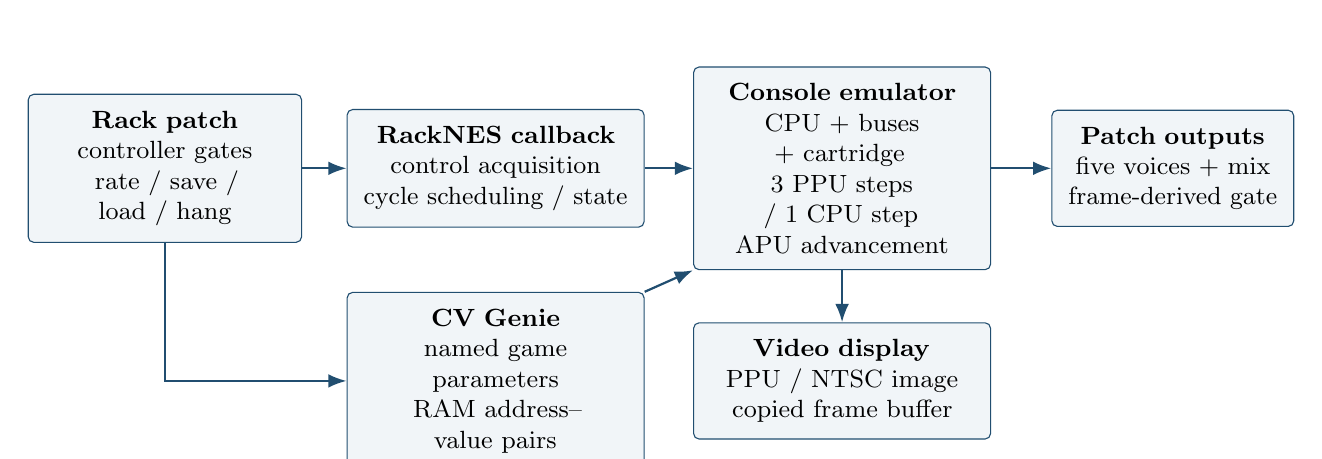
\begin{tikzpicture}[>=Latex,font=\small,
 box/.style={draw=ink,rounded corners=2pt,fill=pale,align=center,inner sep=6pt},
 flow/.style={->,thick,draw=ink}]
\node[box,text width=3.05cm] (patch) at (0,0) {\textbf{Rack patch}\\controller gates\\rate / save / load / hang};
\node[box,text width=3.35cm] (host) at (4.2,0) {\textbf{RackNES callback}\\control acquisition\\cycle scheduling / state};
\node[box,text width=3.35cm] (emu) at (8.6,0) {\textbf{Console emulator}\\CPU + buses + cartridge\\3 PPU steps / 1 CPU step\\APU advancement};
\node[box,text width=2.65cm] (output) at (12.8,0) {\textbf{Patch outputs}\\five voices + mix\\frame-derived gate};
\node[box,text width=3.35cm] (genie) at (4.2,-2.7) {\textbf{CV Genie}\\named game parameters\\RAM address--value pairs};
\node[box,text width=3.35cm] (display) at (8.6,-2.7) {\textbf{Video display}\\PPU / NTSC image\\copied frame buffer};
\draw[flow] (patch) -- (host);
\draw[flow] (host) -- (emu);
\draw[flow] (emu) -- (output);
\draw[flow] (patch.south) |- (genie.west);
\draw[flow] (genie.north east) -- (emu.south west);
\draw[flow] (emu) -- (display);
\end{tikzpicture}
\caption{The host callback advances a coupled console and returns its voices
and a frame-derived gate to the patch. Controller, execution, and memory
interventions enter at different boundaries. State operations act on serialized
emulator components; the diagram does not imply that all host and rendering
state is included in a snapshot.}
\label{fig:architecture}
\end{figure*}

For each host sample, \code{RackNES::process} first handles a pending cartridge
load, acquires divided-rate controls when due, and consumes expander messages.
Unless execution is suspended, it then runs a number of emulator cycles,
updates the frame-derived gate, extracts audio for each voice, and forms the
mix. An emulator cycle calls the PPU three times, the CPU once, and the APU
wrapper once. This follows the NTSC 3:1 PPU-to-CPU relation~\cite{nesclock};
it is a description of the stepping arrangement, not a claim of cycle-accurate
hardware reproduction.

The cartridge layer supports mapper numbers 0--3: NROM, MMC1, UNROM, and CNROM.
That boundary is important for reuse: whole-console control does not imply
support for every cartridge or expansion sound device. Although additional
sound-chip implementations are present in the bundled library, the module
routes the five base NES voices. A program must first work within the
implemented cartridge and machine model before its musical behavior can be
controlled through the patch.

\subsection{Three intervention layers}
At the \emph{gameplay layer}, sixteen gate inputs represent the eight buttons
on each of two controllers. Buttons are combined into bitmaps and delivered
through the emulator's controller interface. A gate therefore retains the
game's interpretation of a press: it may move an object, start a sequence, or
have no effect in the current state. This layer preserves the program's
existing rules as part of the mapping from gesture to sound.

At the \emph{execution layer}, rate, save, load, reset, and hang controls act on
the machine that interprets those gestures. Their effects cut across individual
voices. Rate changes how far the coupled machine advances between host samples;
state recall selects an earlier computational condition from which execution
continues. These operations make temporal structure available without requiring
a separate mapping for every game variable.

At the \emph{memory layer}, CV Genie supplies selected values to RAM locations
named by game-specific maps. This bypasses the need to reach a condition through
ordinary gameplay. The layers can be used together, but they provide different
levels of explanation to a performer: a controller label names an action, an
execution control names a machine operation, and a memory label interprets an
address in a particular program.

\section{Timing and Audio Integration}
\subsection{Requested rate and actual cycle scheduling}
Let $p\in[-4,4]$ be the clock knob, $a\in[-1,1]$ the attenuverter, and $v[n]$
the clock input in volts. The requested rate, before conversion to an integer,
is
\begin{equation}
 \begin{aligned}
 f_r[n]&=f_0\,2^{\clip(p+a\,v[n]/5,-4,4)},\\
 f_0&=1{,}789{,}773\ \mathrm{Hz}.
 \end{aligned}
 \label{eq:rate}
\end{equation}
The nominal range is $f_0/16$ to $16f_0$. With $a=1$, an increase of 5~V
adds one octave to the requested execution rate until clipping occurs. The
clock input therefore has a different scaling from a conventional 1~V/octave
pitch input. Because the CPU, PPU, and APU wrapper advance together, the
control changes the temporal basis of gameplay, graphics, and sound events.
It is not an independent musical-tempo parameter.

The current implementation returns the requested rate as an unsigned integer
and compares an integer loop index against its floating-point quotient by the
host sample rate $F_s$. For a stable positive quotient $q[n]$, the number of
loop iterations is
\begin{equation}
 q[n]=\frac{\lfloor f_r[n]\rfloor}{F_s},
 \qquad N[n]=\ceil{q[n]},
 \label{eq:cycles}
\end{equation}
apart from finite-precision effects in forming $q[n]$. No fractional-cycle
remainder is carried to the next sample. The distinction between requested
rate and executed work is therefore structural: for a constant quotient,
the executed rate is $F_sN$, and its excess over the integer request lies in
$[0,F_s)$ under ideal arithmetic. This is a deduction from the loop, not a
measured timing error. It explains why the knob law alone cannot establish
calibrated pitch or exact console timing.

The controller and save/load/reset/hang inputs are acquired once every sixteen
host samples. They have a control-grid spacing of $16/F_s$; a short pulse
entirely between acquisitions can be missed. Clock-rate CV is read inside the
cycle-loop condition, and expander handling runs each host sample, so the
sixteen-sample divider does not describe all controls. Keeping these cadences
distinct is necessary when reasoning about a patch that combines them.

\subsection{Frame clock and video}
The emulator maintains a counter modulo 29,781 cycles for its frame callback.
The clock output is 10~V during one half of this counter's period and 0~V
during the other half. The same counter requests screen-buffer copies. It
provides a convenient execution-derived clock, but is distinct from the PPU's
own scanline and rendering state. In particular, it should not be interpreted
as the CPU clock itself, despite the port's metadata label, or as a guarantee
of exact video-frame synchronization.

The PPU produces image data that passes through the bundled NTSC filter;
the widget displays the copied image. This visual connection helps preserve
the recognizable game context of the instrument. Screen-copy work also occurs
within the sample-processing path when the emulator counter wraps, tying
display publication to execution without making the display refresh rate the
driver of emulation.

\subsection{Sound rendering and patch-dependent mixing}
RackNES routes each of the APU's two pulse voices, triangle voice, noise voice,
and delta modulation channel to its own Blip\_Buffer. The wrapper ends an
APU frame and each buffer frame after every emulated CPU step. Here a library
``frame'' is a span of sound-emulation time, not a video frame. The buffers'
output sample rate follows the host, while the module sets their source-clock
conversion rate to a fixed 768,000~Hz. That value is distinct from both $f_0$
and its voltage-controlled requested rate.

At extraction, an empty buffer yields zero. Otherwise, the wrapper allocates
a temporary vector, reads all available samples, and returns only the first.
Consequently, the use of band-limited synthesis inside the dependency does not
by itself establish a faithful host-rate output stream. The fixed conversion
clock, advancement count, and extraction policy jointly determine the module's
audio. Treating the control as a simple resampling ratio would conceal this
boundary.

For returned signed sample $s_i[n]$ and channel gain $g_i\in[0,2]$, the
implemented voltage scaling is
\begin{equation}
 y_i[n]=g_i\,\frac{10s_i[n]}{32767}.
\end{equation}
This is a numerical conversion, not a measured peak-to-peak level. Let
$\mathcal U[n]$ contain the voices whose individual output ports are
unconnected, and let $g_m\in[0,2]$ be the mix gain. The mix is
\begin{equation}
 y_m[n]=g_m\sum_{i\in\mathcal U[n]}y_i[n].
 \label{eq:mix}
\end{equation}
Connecting a voice removes it from the mix, so patch topology changes the
mixing rule. A performer can send noise to a separate processor while keeping
the remaining voices together. This linear summation of separated outputs
does not reproduce the NES's coupled nonlinear analog mixer~\cite{nesmixer}.
The resulting interface prioritizes access to individual voices.

\section{State and Memory as Musical Material}
\subsection{Recalling an executable condition}
Save captures one JSON backup of emulator state; load restores that backup.
The serialized components include the cartridge, controllers, CPU, PPU,
APU snapshot, and main and picture buses. Binary data use the bundled
\emph{cpp-base64} implementation~\cite{base64}. The module also stores its
current emulator state and backup in the host's patch serialization, retaining
the cartridge's file path as a dependency.

This mechanism suggests a form of sampling whose object is an executable
condition. Repeatedly requesting load can revisit a passage in a game's
behavior, but the subsequent evolution still depends on the running program
and future inputs. A controller change or RAM intervention after recall can
lead to another trajectory. The useful design distinction is between
restarting a computation and replaying already rendered audio; identical
waveform repetition is not implied.

Operation ordering also matters. During control acquisition, save is handled
before reset, and reset before load. Controller bitmaps are updated afterward.
Thus simultaneous requests have a defined source-level order rather than
being independent actions. Hang is checked after control acquisition and
expander handling. While it prevents further console stepping and output
updates, it still permits these control operations and RAM writes. It holds
the previous output voltages rather than explicitly muting them; a downstream
VCA is the appropriate patch element when silence is required.

The snapshot boundary is incomplete: the emulator's frame counter, rendered
pixel buffers, and Blip\_Buffer contents are not serialized, and the current
serializers have additional field-level omissions and defects documented in
the source notes. Recall therefore revisits program conditions without a
guarantee of restoring audiovisual phase. This boundary matters when a
performance depends on the alignment of recalled events with an external clock.

\subsection{CV Genie and program-specific semantics}
CV Genie provides eight input lanes. Each lane selects a named game parameter.
Numeric parameters linearly map a nominal 0--10~V input into configured byte
ranges, while toggle parameters flip a local boolean on rising edges and send
0 or 1. Numeric inputs are not clamped by this mapping. The expander sends
address--value pairs through
Rack's message buffers. RackNES consumes these pairs and writes the values
directly into its RAM buffer. An address value of zero marks an unused or
consumed message in this protocol.

The built-in maps cover \emph{Super Mario Bros.} and \emph{The Legend of Zelda}.
The latter map is particularly instructive: alongside gameplay variables it
names triangle frequency, rhythm, song, per-voice song position, note duration,
and volume. These labels show how a game-specific music driver can become a
parameter surface for a modular patch. They are interpretations recorded in
the source map, not promises that all values or cartridge revisions behave
musically or even remain playable.

Although the expander's name and manual invoke Game Genie, the implemented
path is direct RAM mutation, not an encoded cartridge-read replacement
mechanism. This distinction is useful to an engineer extending the design:
the module edits mutable program state, and the running game can overwrite
that state again. A control's persistence depends on both the expander's
updates and the program's own writes. Numeric continuity at the input also
does not imply semantic continuity in the game; adjacent byte values can
select unrelated songs, objects, or states.

The available module is the input expander. Code for an Output Genie remains
commented out, and no general game-memory-to-CV output is registered. The
present system therefore supports memory intervention, not a complete
bidirectional memory interface. Its frame-derived gate and audio outputs
remain available for feedback through the surrounding patch.

\section{Design Implications}
\subsection{Coupled time as an expressive control}
RackNES makes the relationship between sound generation and program time
audible and patchable. A slow modulation of the requested execution rate can
affect the progression of a game's sound routines alongside graphics and
gameplay. A conceptual patch sends the same modulation source elsewhere in
the rack while using the frame-derived gate to drive a divider. The result is
a shared source of change between console execution and other modules, with
the timing qualifications of Section~4.

This design makes a practical distinction between \emph{coupling} and
\emph{calibration}. Coupling is present because the subsystems advance through
one stepping boundary. Calibration would require a well-defined relationship
among requested machine time, rendered samples, and output phase. A future
implementation can preserve the first property while improving the second;
they need not be treated as the same requirement.

\subsection{State recall as a branching phrase}
A second conceptual patch saves after a musically useful event, then sends a
divided clock to load. Longer intervals permit more of the program's evolution
before recall; shorter intervals revisit a smaller portion. Adding controller
gates or memory writes changes the conditions following each recall. This
frames the saved state as the beginning of a phrase whose continuation is
computed. It also explains why a saved-state control belongs at the instrument
level: its musical meaning depends on program state, future inputs, and the
recall boundary, not only on the sound chip's oscillator parameters.

The implementation's incomplete snapshot coverage limits repeatability, while
the concept points to a clear engineering responsibility. A documented snapshot
contract should specify machine state, clock phase, rendered audio still in
flight, host control state, and external resources separately. The appropriate
contract depends on whether the intended operation is approximate revisiting,
deterministic continuation, or exact sample replay.

\subsection{Exposing semantics and separating voices}
A third conceptual patch selects a named CV Genie music parameter, supplies
a stepped voltage, and routes one voice to an external effect. It combines
access to a program's musical decisions with access to its resulting sound.
This illustrates why both layers are useful: a memory write can alter which
events are produced, while a downstream processor acts on the voice after
the game has allocated and synthesized it.

For future systems, a memory map is part of the musical interface specification.
Useful metadata would include cartridge identity, address, value domain,
meaning, and the conditions under which the program rewrites the field. A
descriptive label alone cannot express all of these constraints. Making such
assumptions explicit would help transfer maps among projects without treating
one game's internal layout as a general console API.

\section{Engineering Boundaries}
Several architectural choices constrain the present implementation. The
per-sample cycle loop has no fractional accumulator, and its work rises with
the requested rate. Audio extraction allocates temporary storage. State
serialization allocates JSON objects, and restoration invokes the cartridge
loading path, including file access, from the processing callback. Frame
copies also occur there. These are concrete sources of variable callback work;
source inspection alone cannot quantify their cost or establish a real-time
execution guarantee.

A revised implementation could retain the musical interface while carrying
fractional cycle debt, specifying one coherent audio timebase, consuming
rendered samples in sequence, and separating prepared state changes from
file access. Snapshot coverage and serializer correctness would need
explicit treatment before claiming deterministic continuation. Such changes
would also need to account for existing patches that depend on the historical
rate or output behavior. These are engineering directions motivated by the
implementation, not results of an optimization campaign.

The account is limited to the inspected source and documentation. Cartridge
compatibility, hardware fidelity, callback latency, and performance practice
remain outside its scope. The patch structures identify design possibilities;
they are not records of measured or observed performances.

\Needspace{7\baselineskip}
\section{Conclusion}
RackNES treats a running console program as part of a modular musical
instrument. Controller signals act through gameplay, execution controls alter
time and saved conditions, and CV Genie reaches named program variables.
Individual audio outputs then connect that computation to the rest of a patch.
The architecture makes state and temporal coupling central to instrument
design, while its current timing, audio conversion, and serialization expose
the boundaries an engineer must specify. The transferable idea is to make
computation itself available for musical intervention, with clear accounts of
what a control changes, what a snapshot preserves, and how emulated events
become host audio.

\section*{Acknowledgments and Availability}
CV Genie was contributed by \code{@anlexmatos}; its memory-map source credits
the Data Crystal reverse-engineering wiki. The implementation builds on
Amish Naidu and contributors' SimpleNES~\cite{simplenes}, adapted through
the author's nes-py~\cite{nespy}; Shay Green's (blargg's) Nes\_Snd\_Emu,
Blip\_Buffer, and nes\_ntsc~\cite{green,ntsc}; Ren\'e Nyffenegger's
cpp-base64~\cite{base64}; and VCV Rack~\cite{rack}. Source, manuals,
and the report are available from
\href{https://github.com/Kautenja/RackNES}{github.com/Kautenja/RackNES}.
The report's \code{sources.md} records the inspected revision, source locations,
and literature provenance. The source-code license is GPL-3.0-or-later, with
separate artwork and dependency terms recorded in the repository's
\href{https://github.com/Kautenja/RackNES/blob/master/LICENSE.md}{license guide}
and \href{https://github.com/Kautenja/RackNES/blob/master/docs/licenses/THIRD-PARTY.txt}{bundled notices}. Cartridge
images are not supplied with this report.

\balance
\begin{thebibliography}{99}
\small\raggedright
\interlinepenalty=10000
\bibitem{racknes}
C. Kauten and contributors, ``RackNES,'' software, version 2.1.0, 2022.
Source revision \code{e8c99bf86295}.
\href{https://github.com/Kautenja/RackNES/tree/e8c99bf86295318724ef62ad40a17ba6897be696}{Archived source revision};
\href{https://github.com/Kautenja/RackNES/blob/e8c99bf86295318724ef62ad40a17ba6897be696/CHANGELOG.md}{project changelog}.

\bibitem{moog1965}
R. A. Moog, ``Voltage controlled electronic music modules,''
\emph{Journal of the Audio Engineering Society}, vol. 13, no. 3,
pp. 200--206, 1965.
\url{https://aes.org/publications/elibrary-page/?id=1204}.

\bibitem{hunt2002}
A. Hunt, M. M. Wanderley, and M. Paradis, ``The importance of parameter mapping
in electronic instrument design,'' in \emph{Proceedings of the International
Conference on New Interfaces for Musical Expression (NIME)}, pp. 88--93, 2002.
\href{https://doi.org/10.5281/zenodo.1176424}{doi:10.5281/zenodo.1176424}.

\bibitem{goncalves2011}
A. Gon\c{c}alves, ``Towards a voltage-controlled computer control and
interaction beyond an embedded system,'' in \emph{Proceedings of NIME},
pp. 92--95, 2011.
\href{https://doi.org/10.5281/zenodo.1178035}{doi:10.5281/zenodo.1178035}.

\bibitem{collins2007}
K. Collins, ``In the loop: Creativity and constraint in 8-bit video game audio,''
\emph{twentieth-century music}, vol. 4, no. 2, pp. 209--227, 2007.
\href{https://doi.org/10.1017/S1478572208000510}{doi:10.1017/S1478572208000510}.

\bibitem{mcalpine2018}
K. B. McAlpine, \emph{Bits and Pieces: A History of Chiptunes}.
Oxford University Press, 2018.
\href{https://doi.org/10.1093/oso/9780190496098.001.0001}{doi:10.1093/oso/9780190496098.001.0001}.

\bibitem{lsdj}
J. Kotlinski, \emph{Little Sound Dj v9.2.6: Operating Manual}, May 9, 2021.
\url{https://www.littlesounddj.com/lsd/latest/documentation/LSDj_9_2_6.pdf}.

\bibitem{olson2016}
B. Olson, ``Transforming 8-bit video games into musical interfaces via reverse
engineering and augmentation,'' in \emph{Proceedings of NIME},
Brisbane, Australia, pp. 73--77, 2016.
\href{https://doi.org/10.5281/zenodo.1176100}{doi:10.5281/zenodo.1176100}.

\bibitem{soundcraft2013}
M. Cerqueira, S. Salazar, and G. Wang, ``SoundCraft: Transducing StarCraft 2,''
in \emph{Proceedings of NIME}, pp. 243--247, 2013.
\href{https://doi.org/10.5281/zenodo.1178492}{doi:10.5281/zenodo.1178492}.

\bibitem{megamachine}
LOOK MUM NO COMPUTER, ``Gameboy Megamachine,'' project documentation.
Accessed September 30, 2026.
\url{https://www.lookmumnocomputer.com/gameboy-megamachine}.

\bibitem{nesclock}
NESdev contributors, ``Cycle reference chart,'' \emph{NESdev Wiki}.
Accessed September 30, 2026.
\url{https://www.nesdev.org/wiki/Cycle_reference_chart}.

\bibitem{nesmixer}
NESdev contributors, ``APU mixer,'' \emph{NESdev Wiki}.
Accessed September 30, 2026.
\url{https://www.nesdev.org/wiki/APU_Mixer}.

\bibitem{simplenes}
A. Naidu and contributors, ``SimpleNES,'' software and project documentation.
Accessed September 30, 2026.
\url{https://github.com/amhndu/SimpleNES}.

\bibitem{nespy}
C. Kauten and contributors, ``nes-py,'' software and project documentation.
Accessed September 30, 2026.
\url{https://github.com/Kautenja/nes-py}.

\bibitem{green}
S. Green (blargg), ``Blargg's audio libraries,'' author documentation for
Nes\_Snd\_Emu and Blip\_Buffer. Accessed September 30, 2026.
\url{https://www.slack.net/~ant/libs/audio.html}.

\bibitem{ntsc}
S. Green (blargg), ``Blargg's NTSC libraries,'' author documentation for nes\_ntsc.
Accessed September 30, 2026.
\url{https://www.slack.net/~ant/libs/ntsc.html}.

\bibitem{rack}
VCV, ``Plugin API guide,'' \emph{VCV Rack Manual}.
Accessed September 30, 2026.
\url{https://vcvrack.com/manual/PluginGuide}.

\bibitem{base64}
R. Nyffenegger, ``cpp-base64,'' software and project documentation.
Accessed September 30, 2026.
\url{https://github.com/ReneNyffenegger/cpp-base64}.
\end{thebibliography}
\end{document}
